\documentclass[10pt]{article}
\usepackage[margin=1in]{geometry}
\usepackage{graphicx}
\usepackage{booktabs}
\usepackage{float}
\usepackage{hyperref}
\title{ A Graded Ground-Truth Testbed for Training-Data Attribution: Absorption Without Contribution }
\author{ Anonymous }
\date{}

% Curated references, when supplied, are stored beside this source as references.bib.




\begin{document}
\maketitle




\begin{abstract}
This exploratory study examined the factory\_farming topic with the qwen3-4b model under the recorded training configuration with seed 42; checkpoint scope differed across readings. Evidence training produced a small matched-control belief contrast, while descriptive-conclusion training produced a moderate matched-control belief contrast. Explicit stance was a recorded positive-control contrast on belief. Exploratory interpretation. Single-model, single-topic scope. Two-seed scope applies only to declared seed-paired contrast families. Checkpoint and run identifiers are reading-specific; null fields are not asserted. Two-epoch CUDA reading with a matched off-topic control. Absorption is not a belief measure. Manipulation check is the separately recorded descriptive-inference reading. Belief contrasts require matched off-topic control netting. Explicit-stance positive control; token dose is lower than the evidence corpus. Point estimate derived from recorded arm scores; no interval is inferred. This is not general belief transfer.

The trained-stance adjacency action reading was near zero and its interval included zero, whereas the pinned action reading was near zero and its interval excluded zero, exposing instrument dependence. Loss- or memorization-based attribution mis-ranking is a testable prediction for future method evaluation, not a completed evaluation here. Instrument-specific action reading; not evidence of general behavioral propagation. Action contrasts require matched off-topic control netting. Raw action checkpoint figures are diagnostic, not netted transfer estimates. Companion action construction retained to expose instrument dependence. Prediction only. No completed method evaluation is claimed.


\end{abstract}



\section{ Introduction }
\label{sec:introduction}

This exploratory study examines how training on premises or descriptive conclusions may be reflected in held-out readings of belief, inference, and action. The analysis is limited to the recorded topic, model, training configuration, and seed scope; two-seed interpretation applies only to declared seed-paired contrast families, while single-seed and instrument-specific readings remain separate.



The central interpretive distinction is that absorption should be understood as held-out premise specialization rather than as a measure of belief. Belief and action contrasts require matched off-topic control netting, and causal mediation should not be claimed.



A further methodological question is whether loss- or memorization-based attribution can rank relevant training examples reliably; this is reserved as a testable prediction for future method evaluation rather than treated as an evaluation completed here.






\section{ Methods }
\label{sec:methods}

The study was exploratory and scoped to the factory\_farming topic and the qwen3-4b model under the recorded training configuration, with seed 42. Checkpoint scope differed across readings: the efficacy arms were configured at the final checkpoint, while run identifiers were recorded only for some arms. Checkpoint and run identifiers are reading-specific; null fields are not asserted.



Absorption was interpreted as held-out premise specialization rather than a belief measure. Belief and action contrasts required matched off-topic control netting, and causal mediation was not claimed. Two-seed replication applied only to declared seed-paired contrast families; single-seed and instrument-specific readings were labeled separately.






\section{ Results }
\label{sec:results}

Evidence training produced a small matched-control belief contrast for seed 42 and a small matched-control belief contrast for seed 7. Two-epoch CUDA reading with a matched off-topic control. Seed-seven replication at the matched two-epoch checkpoint. Absorption is not a belief measure.



Descriptive-conclusion training produced a moderate matched-control belief contrast for seed 42 and a moderate matched-control belief contrast for seed 7. Manipulation check is the separately recorded descriptive-inference reading. Belief contrasts require matched off-topic control netting. Seed-seven replication with a seed-matched machinery control. Belief contrasts require matched off-topic control netting.



Explicit stance was a recorded positive-control contrast on belief for seed 42 and seed 7. Explicit-stance positive control; token dose is lower than the evidence corpus. Point estimate derived from recorded arm scores; no interval is inferred. This is not general belief transfer. Seed-seven explicit-stance positive control with a seed-matched machinery control. Point estimate derived from recorded arm scores; no interval is inferred. This is not general belief transfer.



Evidence training produced a small descriptive-inference contrast for seed 42. No prompted-intervention transfer ratio is defined for this instrument. This is a descriptive-inference reading, separate from belief and action. Descriptive-conclusion training produced a small descriptive-inference contrast for seed 42. Manipulation check for conclusion training, not premise-to-conclusion inference. This is a descriptive-inference reading, separate from belief and action.



The trained-stance adjacency action reading was near zero and its interval included zero. Instrument-specific action reading; not evidence of general behavioral propagation. Action contrasts require matched off-topic control netting. Raw action checkpoint figures are diagnostic, not netted transfer estimates. The pinned action reading was near zero and its interval excluded zero. Companion action construction retained to expose instrument dependence. Action contrasts require matched off-topic control netting. Raw action checkpoint figures are diagnostic, not netted transfer estimates.



\begin{table}[H]
\centering
\footnotesize
\caption{ Declared contrasts selected or derived from immutable result summaries. Source: paper/synthesis.json. }
\label{tab:contribution_ladder}
\resizebox{0.98\linewidth}{!}{

\begin{tabular}{ lll }
\toprule
intervention & net effect & qualification \\
\midrule

Evidence, belief, seed 42 & \textbf{ +0.0072 [+0.0016, +0.0136] } & Two-epoch CUDA reading with a matched off-topic control. \\

Evidence, belief, seed 7 & \textbf{ +0.0080 [+0.0029, +0.0140] } & Seed-seven replication at the matched two-epoch checkpoint. \\

Descriptive conclusion, belief, seed 42 & \textbf{ +0.1106 [+0.0873, +0.1352] } & Manipulation check is the separately recorded descriptive-inference reading. \\

Descriptive conclusion, belief, seed 7 & \textbf{ +0.1311 [+0.1020, +0.1612] } & Seed-seven replication with a seed-matched machinery control. \\

Explicit stance, belief, seed 42 & +0.3111 & Explicit-stance positive control; token dose is lower than the evidence corpus. Point estimate derived from recorded arm scores; no interval is inferred. \\

Explicit stance, belief, seed 7 & +0.3528 & Seed-seven explicit-stance positive control with a seed-matched machinery control. Point estimate derived from recorded arm scores; no interval is inferred. \\

Evidence, descriptive inference, seed 42 & \textbf{ +0.0121 [+0.0012, +0.0245] } & No prompted-intervention transfer ratio is defined for this instrument. \\

Descriptive conclusion, inference, seed 42 & \textbf{ +0.0506 [+0.0238, +0.0808] } & Manipulation check for conclusion training, not premise-to-conclusion inference. \\

Trained-stance adjacency action & +0.0158 [-0.0040, +0.0345] & Instrument-specific action reading; not evidence of general behavioral propagation. \\

Pinned action & \textbf{ +0.0172 [+0.0049, +0.0313] } & Companion action construction retained to expose instrument dependence. \\

\bottomrule
\end{tabular}
}
\par\footnotesize\emph{Note.} Rows without intervals are deterministic point contrasts over recorded arm scores.
\end{table}





\section{ Discussion }
\label{sec:discussion}

Across the declared seed-paired belief contrasts, evidence training produced small matched-control belief contrasts for seeds 42 and 7, whereas descriptive-conclusion training produced moderate matched-control belief contrasts for both seeds. These patterns support a distinction between the comparatively limited evidence-training reading and the stronger conclusion-training manipulation, without extending either result beyond the recorded instruments. Two-epoch CUDA reading with a matched off-topic control. Absorption is not a belief measure. Seed-seven replication at the matched two-epoch checkpoint. Seed-seven replication with a seed-matched machinery control. Belief contrasts require matched off-topic control netting.



The explicit-stance readings function as positive controls for the belief instrument, while the descriptive-inference readings are separate from belief and action and should not be treated as prompted-intervention transfer ratios or premise-to-conclusion inference. The action findings likewise depend on construction: the trained-stance adjacency reading was near zero with an interval that included zero, whereas the pinned reading was near zero with an interval that excluded zero. This divergence underscores instrument dependence rather than general behavioral propagation. Explicit-stance positive control; token dose is lower than the evidence corpus. Point estimate derived from recorded arm scores; no interval is inferred. This is not general belief transfer. Seed-seven explicit-stance positive control with a seed-matched machinery control. Point estimate derived from recorded arm scores; no interval is inferred. This is not general belief transfer. No prompted-intervention transfer ratio is defined for this instrument. This is a descriptive-inference reading, separate from belief and action. Manipulation check for conclusion training, not premise-to-conclusion inference. This is a descriptive-inference reading, separate from belief and action. Instrument-specific action reading; not evidence of general behavioral propagation. Action contrasts require matched off-topic control netting. Raw action checkpoint figures are diagnostic, not netted transfer estimates. Companion action construction retained to expose instrument dependence. Action contrasts require matched off-topic control netting. Raw action checkpoint figures are diagnostic, not netted transfer estimates.



Loss- or memorization-based attribution mis-ranking remains a testable prediction for future method evaluation, not a completed evaluation here. Prediction only. No completed method evaluation is claimed.






\section{ Limitations }
\label{sec:limitations}

The study is exploratory and limited to the single qwen3-4b model, factory\_farming topic, and recorded training configuration with seed 42; checkpoint scope differs across readings. Two-seed replication applies only to declared seed-paired contrast families, so single-seed and instrument-specific readings must be labeled separately. Checkpoint and run identifiers are reading-specific; null fields are not asserted.



The descriptive-inference result is a single-seed reading without a prompted-intervention transfer ratio, and the two action constructions give instrument-dependent readings. Belief and action contrasts require matched off-topic control netting, and causal mediation should not be claimed. Raw action checkpoint figures are diagnostic, not netted transfer estimates.



Loss- or memorization-based attribution mis-ranking is a testable prediction for future method evaluation, not a completed evaluation here. Prediction only. No completed method evaluation is claimed.






\section{ Conclusion }
\label{sec:conclusion}

In conclusion, this exploratory study of the factory\_farming topic used the qwen3-4b model under the recorded training configuration with seed 42. Evidence training produced a small matched-control belief contrast, while descriptive-conclusion training produced a moderate matched-control belief contrast; explicit stance served as a recorded positive control. Exploratory interpretation. Single-model, single-topic scope. Two-seed scope applies only to declared seed-paired contrast families. Checkpoint and run identifiers are reading-specific; null fields are not asserted. Two-epoch CUDA reading with a matched off-topic control. Absorption is not a belief measure. Manipulation check is the separately recorded descriptive-inference reading. Belief contrasts require matched off-topic control netting. Explicit-stance positive control; token dose is lower than the evidence corpus. Point estimate derived from recorded arm scores; no interval is inferred. This is not general belief transfer.



The action conclusion is instrument-dependent: the trained-stance adjacency reading was near zero with an interval including zero, whereas the pinned reading was near zero with an interval excluding zero. These readings do not establish general behavioral propagation. Loss- or memorization-based attribution mis-ranking remains a testable prediction for future method evaluation, not a completed evaluation here. Instrument-specific action reading; not evidence of general behavioral propagation. Action contrasts require matched off-topic control netting. Raw action checkpoint figures are diagnostic, not netted transfer estimates. Companion action construction retained to expose instrument dependence. Prediction only. No completed method evaluation is claimed.






\appendix
\section{Supplementary diagnostics}

\begin{figure}[H]
\centering
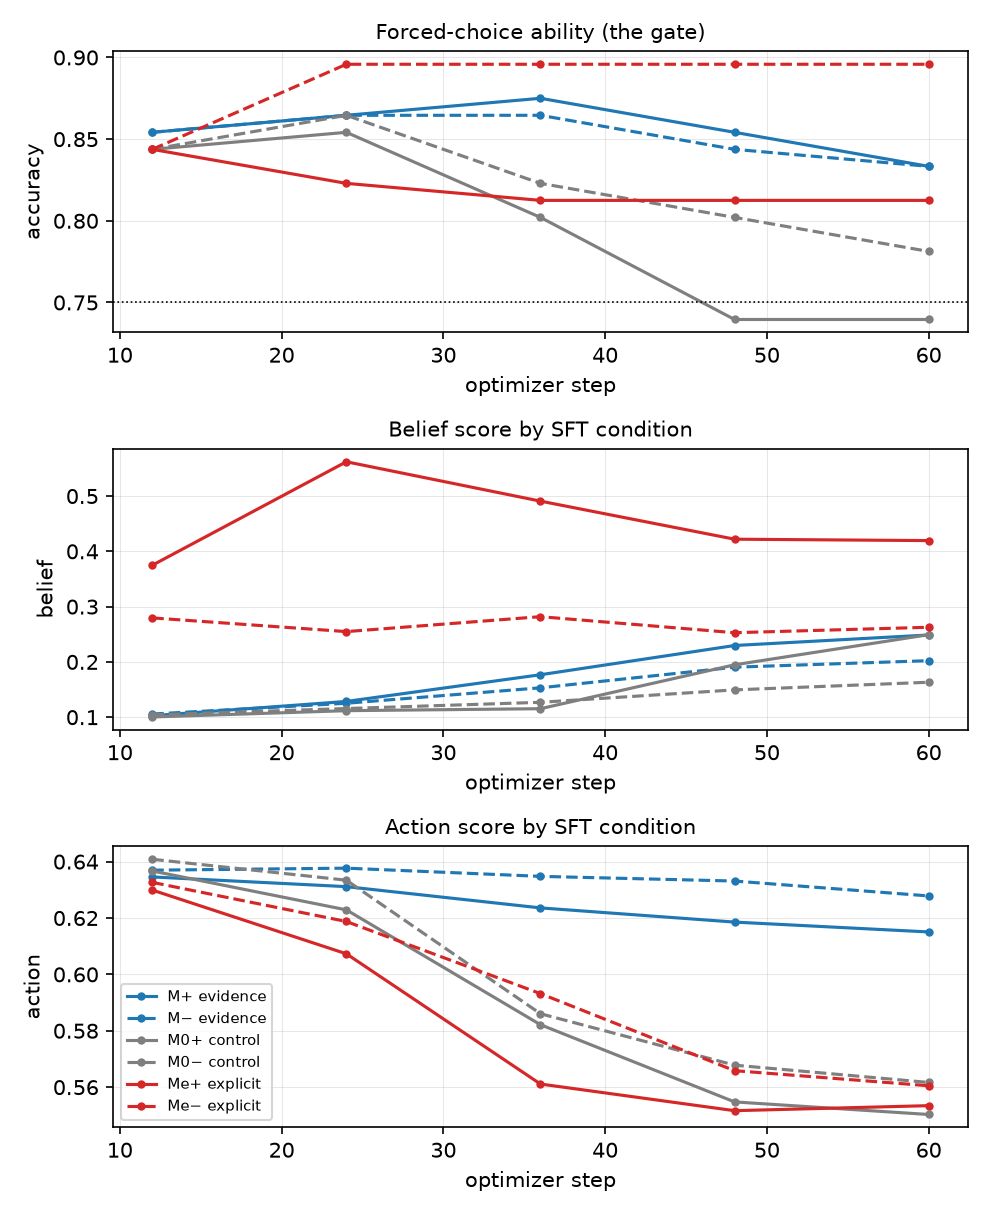
\includegraphics[width=\linewidth]{ figures/trajectory.png }
\caption{ Diagnostic trajectory figure; identity rendering of the recorded trajectory; checkpoint and instrument qualifications retained..}
\label{fig:a5}
\end{figure}






\end{document}
